\documentclass[10pt,landscape,letterpaper]{article}
\usepackage[utf8]{inputenc}
\usepackage[ngerman]{babel}
\usepackage[T1]{fontenc}
\usepackage{lmodern}
%\usepackage[LY1,T1]{fontenc}
%\usepackage{frutigernext}
%\usepackage[lf,minionint]{MinionPro}
\usepackage{tikz}
\usetikzlibrary{shapes,positioning,arrows,fit,calc,graphs,graphs.standard}
\usepackage[nosf]{kpfonts}
\usepackage[t1]{sourcesanspro}
\usepackage{multicol}
\usepackage{wrapfig}
\usepackage[top=4mm,bottom=4mm,left=4mm,right=4mm]{geometry}
\usepackage[framemethod=tikz]{mdframed}
\usepackage{microtype}
\usepackage{pdfpages}
\usepackage{lipsum}
% https://tex.stackexchange.com/a/112573
\usepackage[most]{tcolorbox}
\usepackage{etoolbox}
\usepackage{listings}
\usepackage{realboxes}

% https://tex.stackexchange.com/a/39785
% https://tex.stackexchange.com/a/42081/228904
\usepackage{circuitikz}
\usetikzlibrary{arrows.meta}
\usepackage{siunitx}

\usepackage{graphicx}
\graphicspath{ {./images/} }

\let\bar\overline

\definecolor{myblue}{cmyk}{1,.72,0,.38}

\def\firstcircle{(0,0) circle (1.5cm)}
\def\secondcircle{(0:2cm) circle (1.5cm)}

\colorlet{circle edge}{myblue}
\colorlet{circle area}{myblue!5}

\tikzset{filled/.style={fill=circle area, draw=circle edge, thick},
    outline/.style={draw=circle edge, thick}}
    
\pgfdeclarelayer{background}
\pgfsetlayers{background,main}

\everymath\expandafter{\the\everymath \color{myblue}}
\everydisplay\expandafter{\the\everydisplay \color{myblue}}

\renewcommand{\baselinestretch}{.8}
\pagestyle{empty}

\global\mdfdefinestyle{header}{%
linecolor=gray,linewidth=1pt,%
leftmargin=0mm,rightmargin=0mm,skipbelow=0mm,skipabove=0mm,
}

\newcommand{\header}{
\begin{mdframed}[style=header]
\footnotesize
\sffamily
Hilfszettel zur Klausur\\
von~Tim~S.,~Seite~\thepage~von~2
\end{mdframed}
}

% more compact minted custom frames
\newtcolorbox{mintedbox}[1][]
{
  colframe = black!20,
  colback  = white,
  left = 0pt,
  right = 0pt,
  top = 0pt,
  bottom = 0pt,
  #1,
}

% make code font smaller
\setminted{fontsize=\footnotesize}

% nicer frame for minted environments
\BeforeBeginEnvironment{minted}{\begin{mintedbox}}%
\AfterEndEnvironment{minted}{\end{mintedbox}}%


\makeatletter % Author: https://tex.stackexchange.com/questions/218587/how-to-set-one-header-for-each-page-using-multicols
\renewcommand{\section}{\@startsection{section}{1}{0mm}%
                                {.2ex}%
                                {.2ex}%x
                                {\color{myblue}\sffamily\normalsize\bfseries}}
\renewcommand{\subsection}{\@startsection{subsection}{1}{0mm}%
                                {.2ex}%
                                {.2ex}%x
                                {\sffamily\bfseries}}



% \def\multi@column@out{%
%    \ifnum\outputpenalty <-\@M
%    \speci@ls \else
%    \ifvoid\colbreak@box\else
%      \mult@info\@ne{Re-adding forced
%                break(s) for splitting}%
%      \setbox\@cclv\vbox{%
%         \unvbox\colbreak@box
%         \penalty-\@Mv\unvbox\@cclv}%
%    \fi
%    \splittopskip\topskip
%    \splitmaxdepth\maxdepth
%    \dimen@\@colroom
%    \divide\skip\footins\col@number
%    \ifvoid\footins \else
%       \leave@mult@footins
%    \fi
%    \let\ifshr@kingsaved\ifshr@king
%    \ifvbox \@kludgeins
%      \advance \dimen@ -\ht\@kludgeins
%      \ifdim \wd\@kludgeins>\z@
%         \shr@nkingtrue
%      \fi
%    \fi
%    \process@cols\mult@gfirstbox{%
% %%%%% START CHANGE
% \ifnum\count@=\numexpr\mult@rightbox+2\relax
%           \setbox\count@\vsplit\@cclv to \dimexpr \dimen@-1cm\relax
% \setbox\count@\vbox to \dimen@{\vbox to 1cm{\header}\unvbox\count@\vss}%
% \else
%       \setbox\count@\vsplit\@cclv to \dimen@
% \fi
% %%%%% END CHANGE
%             \set@keptmarks
%             \setbox\count@
%                  \vbox to\dimen@
%                   {\unvbox\count@
%                    \remove@discardable@items
%                    \ifshr@nking\vfill\fi}%
%            }%
%    \setbox\mult@rightbox
%        \vsplit\@cclv to\dimen@
%    \set@keptmarks
%    \setbox\mult@rightbox\vbox to\dimen@
%           {\unvbox\mult@rightbox
%            \remove@discardable@items
%            \ifshr@nking\vfill\fi}%
%    \let\ifshr@king\ifshr@kingsaved
%    \ifvoid\@cclv \else
%        \unvbox\@cclv
%        \ifnum\outputpenalty=\@M
%        \else
%           \penalty\outputpenalty
%        \fi
%        \ifvoid\footins\else
%          \PackageWarning{multicol}%
%           {I moved some lines to
%            the next page.\MessageBreak
%            Footnotes on page
%            \thepage\space might be wrong}%
%        \fi
%        \ifnum \c@tracingmulticols>\thr@@
%                     \hrule\allowbreak \fi
%    \fi
%    \ifx\@empty\kept@firstmark
%       \let\firstmark\kept@topmark
%       \let\botmark\kept@topmark
%    \else
%       \let\firstmark\kept@firstmark
%       \let\botmark\kept@botmark
%    \fi
%    \let\topmark\kept@topmark
%    \mult@info\tw@
%         {Use kept top mark:\MessageBreak
%           \meaning\kept@topmark
%          \MessageBreak
%          Use kept first mark:\MessageBreak
%           \meaning\kept@firstmark
%         \MessageBreak
%          Use kept bot mark:\MessageBreak
%           \meaning\kept@botmark
%         \MessageBreak
%          Produce first mark:\MessageBreak
%           \meaning\firstmark
%         \MessageBreak
%         Produce bot mark:\MessageBreak
%           \meaning\botmark
%          \@gobbletwo}%
%    \setbox\@cclv\vbox{\unvbox\partial@page
%                       \page@sofar}%
%    \@makecol\@outputpage
%      \global\let\kept@topmark\botmark
%      \global\let\kept@firstmark\@empty
%      \global\let\kept@botmark\@empty
%      \mult@info\tw@
%         {(Re)Init top mark:\MessageBreak
%          \meaning\kept@topmark
%          \@gobbletwo}%
%    \global\@colroom\@colht
%    \global \@mparbottom \z@
%    \process@deferreds
%    \@whilesw\if@fcolmade\fi{\@outputpage
%       \global\@colroom\@colht
%       \process@deferreds}%
%    \mult@info\@ne
%      {Colroom:\MessageBreak
%       \the\@colht\space
%               after float space removed
%               = \the\@colroom \@gobble}%
%     \set@mult@vsize \global
%   \fi}

\makeatother
\setlength{\parindent}{0pt}

\begin{document}
%\footnotesize
\small
\begin{multicols*}{5}
\section{Quick Facts}
\subsection*{Miscellaneous Tips}
\footnotesize
\blockquote{A DNS server using UDP will query a different authoritative
server if its first query is lost (assuming there are multiple
authoritative servers). It attempts to maximize hit probability.}

\blockquote{A TCP handshake takes 1 RTT}

\blockquote{\textbf{Fast retransmission} requires 3 packets losses to be
triggered, and it halves the cwnd. \textbf{Slow retransmission} waits
for the recovery timer to expire and resets the cwnd}

\blockquote{\textbf{Stub resolver} must know the IP address of a caching
resolver. These are usually are the end users.}

\blockquote{\textbf{Cache resolvers} must know the IP address of a root
server.}

\blockquote{\textbf{Authoritative server} the final source of truth
(either address or CNAME).}

\small
\subsection*{Internet Protocol Stack}
\begin{itemize}
  \item \textbf{application}: DNS, FTP, SMTP, HTTP
  \item \textbf{transport}: TCP, UDP
  \item \textbf{network}: IP
  \item \textbf{link}: ethernet, WiFi
\end{itemize}
\subsection*{Stateless Protocols}
\begin{itemize}
  \item HTTP/1.1
  \item DNS
  \item UDP
\end{itemize}
\subsection*{Stateful Protocols}
\begin{itemize}
  \item TCP
\end{itemize}
\subsection*{Has re-trans. timers}
\begin{itemize}
  \item DNS caching resolver
  \item TCP data sender
\end{itemize}
\subsection*{DOESN'T have re-trans. Timers}
\begin{itemize}
  \item HTTP client/server
  \item DNS auth. server
  \item TCP data receiver
\end{itemize}
\subsection*{Common HTTP responses}
\begin{itemize}
  \item 200 OK: request succeeded
  \item 301 Moved Permanently: object moved to a location specified in the message
  \item 400 bad request: message not understood by server
  \item 505 HTTP version not supported
\end{itemize}
\subsection*{HTTP/1.0}
It uses TCP. Allows 1 request per connection. Each request needs to
reopen a connection. Allows parallel connections. Does not allow
pipelining
\subsection*{HTTP/1.1}
It uses TCP. Connection is persistent. As many requests per connection.
Allows pipelining and parallel connections.
\subsection*{HTTP/2.0}
Similar to HTTP/1.1 but it brakes down large packets into frames. This
allows to prevent some forms of head-of-line blocking (cannot prevent
inherent TCP HoL blocking). It also allows to send multiple streams of
data for multiplexing.
\subsection*{HTTP Packet Types}
\resizebox{5cm}{!}{
  \begin{tabular}{ |l|l|l|l|l|l|l| }
    \hline
    \multicolumn{1}{|c|}{Type} & \multicolumn{1}{|c|}{HTTP/1.0} & \multicolumn{1}{|c|}{HTTP/1.1} \\
    \hline
    GET    & yes      & yes \\
    \hline
    POST   & yes      & yes \\
    \hline
    HEAD   & yes      & yes \\
    \hline
    PUT    & no       & yes \\
    \hline
    DELETE & no       & yes \\
    \hline
  \end{tabular}
}
\subsection*{TCP + TLS}
\begin{center}
  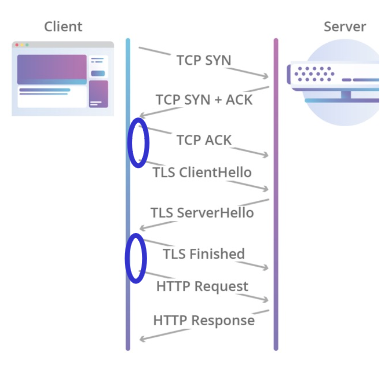
\includegraphics[scale=0.4]{images/tcp-n-tls.png}
\end{center}
\subsection*{Go-Back-N}
Sender has sliding window and can send many unacknowledged packets.
Acknowledgement is for the latest received packet w/o error and sender
window slides. On packet loss it retransmits all packets in the sliding
window. ACKs are cumulative. It does not buffers packets.
\subsection*{Selective Repeat}
Sender has sliding window and can send many unacknowledged packets.
Receiver acknowledges each received packet, and it buffers them
(out-of-order if necessary). Sender "selects" ACKed packets and re-sends
unACKed ones when their individual timers expire.
\section{Equations}
\subsection*{Voltage Divider}
$V_o = \frac{R_2}{R_1+R_2}\cdot V_s$
\begin{center}
  \begin{circuitikz}[
    american, scale = 0.8, transform shape
  ]
    \ctikzset{
      batteries/scale=0.7,
      resistors/scale=0.55,
      % font=\footnotesize
    }
    \draw
      (0,0) to[battery, invert, l=$V_s$] ++(0,3)
      to[short] ++(1,0)
      to[R, l_=$R_1$] ++(0,-1.5) coordinate (vp)
      to[R, l_=$R_2$] ++(0,-1.5) coordinate (vn)
      to[short] ++(-1,0)
      (vp) to[short, *-o] ++(1,0) coordinate (vpl)
      (vn) to[short, *-o] ++(1,0) coordinate (vnl)
    ;
    \node at ($(vpl)!0.5!(vnl)$) {$V_o$};
  \end{circuitikz}
\end{center}

\subsection*{AC Current}
To compute impedances\\
$Z_C=\frac{1}{j\omega C},~~Z_L=j\omega L$\\
To compute frequency\\
$f=\omega/2\pi$
\subsection*{Power}
$P=IV=\frac{V^2}{R}$
\subsection*{Resonant Frequency}
For $\omega_0$, $X_L=X_C$\\
$\omega_0L=\frac{1}{\omega_0C}$\\
solve for $\omega_0$ and then
$f_0=\frac{\omega_0}{2\pi}$
\section{Circuits}
\subsection*{Switch with Transients 1}
It's been a long time. All transients have died out.
\begin{center}
  \begin{circuitikz}[
    american, scale = 0.6, transform shape
  ]
    \ctikzset{
      batteries/scale=0.7,
      resistors/scale=0.55,
      capacitors/scale=0.6,
      bipoles/cuteswitch/thickness=0.3
      % font=\footnotesize
    }
    \draw
      (0,0) to[battery, l_=$\qty{28}{\volt}$] ++(0,2)
      to[R, l=$\qty{4}{\kilo\ohm}$] ++(2,0)
      % to[short] ++(1,0)
      to[cute opening switch, invert, name=swlbl] ++(1,0) coordinate(swtch)
      to[cute inductor,l^=$\qty{200}{\milli\henry}$] ++(0,-2) coordinate(lpbck1)
      -- (0,0)
    ;
    \draw[draw=black, dash pattern=on 1pt off 1pt]
      (swlbl.in) to[short] ++(0,0.75) coordinate(swdash)
    ;
    \draw
      (swdash) to[short, o-] ++(0,0.5)
      to[R, l=$\qty{24}{\kilo\ohm}$] ++(2,0)
      to[short, -*] ++(0,-1.25)
      to[curved capacitor,l=$\qty{8}{\nano\farad}$] ++(2,0)
      to[battery, l=$\qty{20}{\volt}$] ++(0,-2)
      to[short, -*] (lpbck1)
      (swlbl.in) to[R, l=$\qty{12}{\kilo\ohm}$] ++(2,0)
    ;
    \node[below] at (swlbl.out){a};
    \node[left] at (swdash){b};
  \end{circuitikz}
\end{center}
At $t=0^-$ for the capacitor current thru is 0 and voltage across is
\qty{20}{\volt} (higher to the right). For the inductor current thru is
\qty{7}{mA} (updward) and voltage across is 0.

At $t=0^+$ for the capacitor current thru is \qty{7}{mA} (left-to-right)
and voltage across is preserved. For the inductor current thru is
preserved and voltage across is \qty{56}{\volt} (higher at the top)
given by\\
\begin{scriptsize}
  $V_C(0^+) + \qty{20}{\volt} - V_L(0^+) + \qty{8}{\kilo\ohm}(\qty{7}{\milli\ampere})=0.$
\end{scriptsize}\\
The capacitor voltage at $0^+$ is \qty{20}{\volt} which is negative for a CW KVL, so only the
last term remains and we get \qty{56}{\volt}.

\subsection*{Second Order Circuit}
\begin{center}
  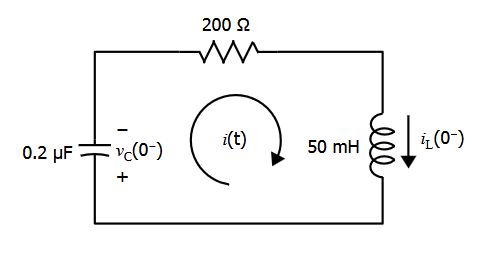
\includegraphics[scale=0.4]{second-order-final-pp.png}
\end{center}
This is a second-order circuit. There is an initial voltage on the
capacitor (assuming clockwise current) $v(0^-)=+\qty{12}{\volt}$, and an
initial current in the inductor $i_L(0^-)=\qty{30}{\milli\ampere}$
clockwise. In order to solve the differential equation for $i(t)$, the
initial voltages $v_L(0^+)$ and $v_R(0^+)$, and
$\left.\frac{d}{dt}i(t)\right\vert_{t=0^+}$ must be found. Using what
you know about inductors, capacitors, and KCL, find these values.\\
\begin{scriptsize}
  $i\left(0^+\right)=i_L\left(0^-\right)=\qty{30}{\milli\ampere}$\\
  $v_C\left(0^+\right)=v_C\left(0^-\right)=\qty{12}{\volt}$\\
  $v_R\left(0^+\right)=i\left(0^+\right)R=\qty{6}{\volt},~\text{+ to left}$\\
  $\text{KVL at }t=0^+:~+6+12+v_L\left(0^+\right)=0$\\
  $v_L\left(0^+\right)=\qty{-18}{\volt},~\text{+ at bottom}$\\
  since $v_L\left(0^+\right)=L\left.\frac{d}{dt}i\left(t\right)\right\vert_{t=0^+}$\\
  $\left.\frac{d}{dt}i\left(t\right)\right\vert_{t=0^+}=\frac{v_L\left(0^+\right)}{L}=-\qty{360}{\ampere\per\second}$\\
\end{scriptsize}

\subsection*{Max Power Transfer}
\begin{center}
  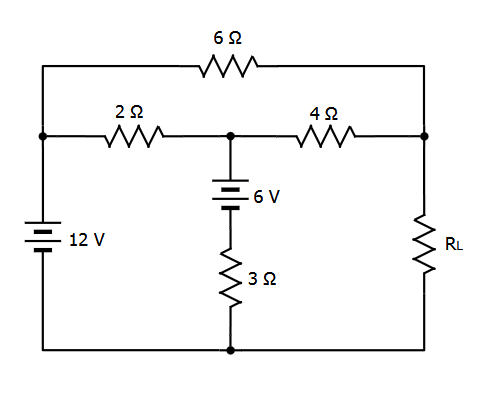
\includegraphics[scale=0.4]{max-power-final-pp.png}
\end{center}
Find the value of $R_L$ for maximum power transfer to $R_L$. First, Find
Thevenin Equiv Resistance.

Setup system for open circuit voltage (assume $R_L$ is not there)\\
\begin{scriptsize}
  $V_{1}=12$\\
  $\frac{V_{2}-12}{2}+\frac{V_{2}-6}{3}+\frac{V_{2}-V_{OC}}{4}=0$\\
  $\frac{V_{OC}-V_{2}}{4}+\frac{V_{OC}-12}{6}=0$\\
\end{scriptsize}
Solve system\\
\begin{scriptsize}
  $V_{2}\approx\qty{9.8571}{\volt}$\\
  $V_{OC}\approx\qty{10.7143}{\volt}$\\
\end{scriptsize}
Setup system for short circuit current (assume $R_L$ is a short). $V_3$
is the same node that $V_2$ were\\
\begin{scriptsize}
  $\frac{V_{3}-12}{2}+\frac{V_{3}-6}{3}+\frac{V_{3}}{4}=0$\\
\end{scriptsize}
Solve system\\
$V_{3}=\qty{7.3846}{\volt}$\\
Now compute currents thru \qty{6}{\ohm} and \qty{4}{\ohm} resistors\\
\begin{scriptsize}
  $I_{4}=\frac{V_{1}}{4}=\qty{1.8462}{\ampere}$\\
  $I_{6}=\frac{12}{6}   =\qty{2}{\ampere}$\\
\end{scriptsize}
By KCL\\
$I_{SC}=I_{4}+I_{6}=\qty{3.8462}{\ampere}$\\
Finally\\
$R_{L}=R_{th}=\frac{V_{OC}}{I_{SC}}=\qty{2.79}{\ohm}$

\subsection*{Output Impedance 1}
\begin{center}
  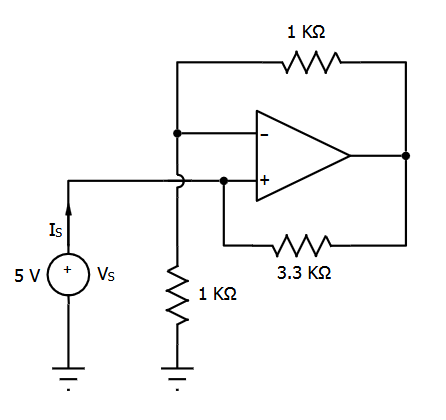
\includegraphics[scale=0.4]{op-amp-final-pp.png}
\end{center}
Setup system from nodes\\
\begin{scriptsize}
  $\frac{v_n}{\qty{1}{\kilo\ohm}} + \frac{v_n-v_{oa}}{\qty{1}{\kilo\ohm}} = 0$\\
  $\frac{v_p - v_{oa}}{\qty{3.3}{\kilo\ohm}} - I_S = 0$\\
\end{scriptsize}
Solve system\\
$v_{oa} = \qty{10}{\volt};~~I_S\approx\qty{-1.515}{\milli\ampere}$\\
Finally\\
$R_{in} \approx \frac{\qty{5}{\volt}}{\qty{-1.515}{\milli\ampere}} = \qty{-3.3}{\kilo\ohm}$

\subsection*{Dependent Sources}
\begin{center}
  \begin{circuitikz}[american, scale = 0.625, transform shape]
    \ctikzset{
      inductors/scale=1,
      sources/scale=0.75,
      csources/scale=0.75,
      resistors/scale=0.625,
      capacitors/scale=0.625
    }
    % x: 7 divs (1 unit each), y: 2.5 divs (1 unit each)
    \draw
      (1,2.5) to[R=$\qty{10}{\ohm}$, *-] ++(0,-1.5) % res 10 ohm
      to[short, -*] ++(0,-1) % res 10 ohm
      to[short] ++(-1,0) % short
      to[isource, l_=$10.6\Angle\qty{0}{\degree}\unit{\ampere}$] ++(0,1.5) % curr src 10.6 ang 0 deg
      to[short] ++(0,1) % short
      to[short] ++(1,0) % short
      to[R=$\qty{1}{\ohm}$] ++(2,0) % res 1 ohm
      to[cute inductor,i>_=$i_x$,l^=$j\qty{2}{\ohm}$] ++(2,0) % indc j2 ohm
      to[curved capacitor,l_=$-j\qty{5}{\ohm}$, *-*] ++(0,-2.5) % cap -j5 ohm
      to[short] ++(2,0) % short
      to[cV,l=$\qty{20}{\ohm}i_x$, invert] ++(0,2.5) % dep volt src 20 * i_x
      to[R=$\qty{5}{\ohm}$] ++(-2,0) % res 5 ohm
      (1,0) to[short] ++(4,0) % short
    ;
    \node[above] at (1,2.5){$v_1$};
    \node[above] at (5,2.5){$v_2$};
  \end{circuitikz}
\end{center}
First simplify series impedance\\
$\Rightarrow\qty{1}{\ohm}+j\qty{2}{\ohm} = \acimp{\sqrt{5}}{\arctan(2)}$\\
Then set KCL\\
\begin{scriptsize}
  $\text{node at }v_1 : \acamp{-10.6}{0} + \frac{v_1}{\qty{10}{\ohm}} + i_x = \qty{0}{\ampere}$ \\
  $\text{node at }v_2 : -i_x + \frac{v_2}{-\acimp{5}{90}} + \frac{v_2-\qty{20}{\ohm}i_x}{\qty{5}{\ohm}} = \qty{0}{\ampere}$\\
\end{scriptsize}
also\\
$i_x = \frac{v_1-v_2}{\acimp{\sqrt{5}}{\arctan(2)}}$\\
Solve system.

\subsection*{Op Amp Example 1}
\begin{center}
  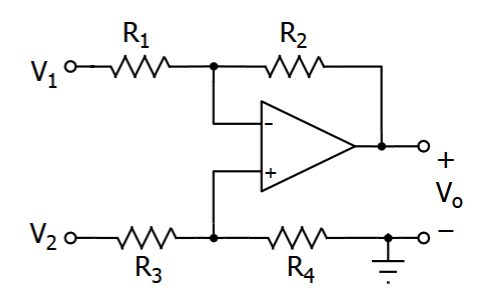
\includegraphics[scale=0.4]{op-amp-simpl-1.png}
\end{center}
Assume that $R_1=R_3$ and $R_2=R_4$, then\\
$V_O=\frac{R_2}{R_1}\left(V_2-V_1\right)$
\subsection*{Switched Capacitor}
\begin{center}
  \begin{circuitikz}[american, scale = 0.6, transform shape]
    \ctikzset{bipoles/cuteswitch/thickness=0.4}
    \draw
    (0,0) to[battery, l=5V, invert] (0,3) % Battery
    to[cute closing switch, name=Sw] (3,3) % Switch
    to[R=$\qty{10}{\ohm}$] (6,3) % Resistor
    to[curved capacitor,l=$\qty{1}{\micro\farad}$, name=Cap] (6,0) % Capacitor with voltage label
    -- (0,0); % Ground connection
    \node[below] at (Sw){$t=0$};
    \node[left=0.5cm] at (Cap){$v_C(0^-)=\qty{2}{\volt}$};
  \end{circuitikz}
\end{center}
Equation is $v_C(t) = V_s + Ke^{-\frac{t}{RC}}$\\
in case you need it diff. eqn. is\\
$\frac{d}{dt}v_C(t)+\frac{v_C(t)}{RC} = \frac{V_s}{RC}$ \\
Plug and chug you get $K = \boxed{\qty{-3}{\volt}}$. And in equation
form\\
$v_C(t) = \boxed{\qty{5}{\volt} + (\qty{-3}{\volt})e^{-\frac{t}{\qty{10}{\micro\second}}}}$
\section{SI}
\subsection*{Units}
Power: $\unit{\watt}=\unit{\joule\per\second}=\unit{\volt\ampere}$\\
Charge: $\unit{\coulomb}=\unit{\ampere\second}=\unit{\farad\volt}$\\
Capacitance: $\unit{\farad}=\unit{\coulomb\per\volt}=\unit{\second\per\ohm}$\\
Inductance: $\unit{\henry}=\unit{\volt\second\per\ampere}$\\
Voltage: $\unit{\volt}=\unit{\watt\per\ampere}=\unit{\joule\per\coulomb}$\\
Resistance: $\unit{\ohm}=\unit{\volt\per\ampere}$\\
Current: $\unit{\ampere}=\unit{\farad\volt\per\second}$
\subsection*{Prefixes}
$\text{pico}=\num{e-12}$\\
$\text{nano}=\num{e-9}$\\
$\text{micro}=\num{e-6}$\\
$\text{milli}=\num{e-3}$\\

\end{multicols*}
\end{document}